\documentclass[border=1cm]{standalone}
\usepackage{tikz}
\usetikzlibrary{math}
% Define a equilateral triangle with lower left corner at coordinate #1 and
% with length of the sides #2
\newcommand\Triangle[2]{
\draw #1 coordinate(a) -- ++(0:#2) coordinate(b) ;
\draw (a) -- ++(60:#2) coordinate(c);
\fill (a) -- (b) -- (c) -- cycle;
}
\begin{document}
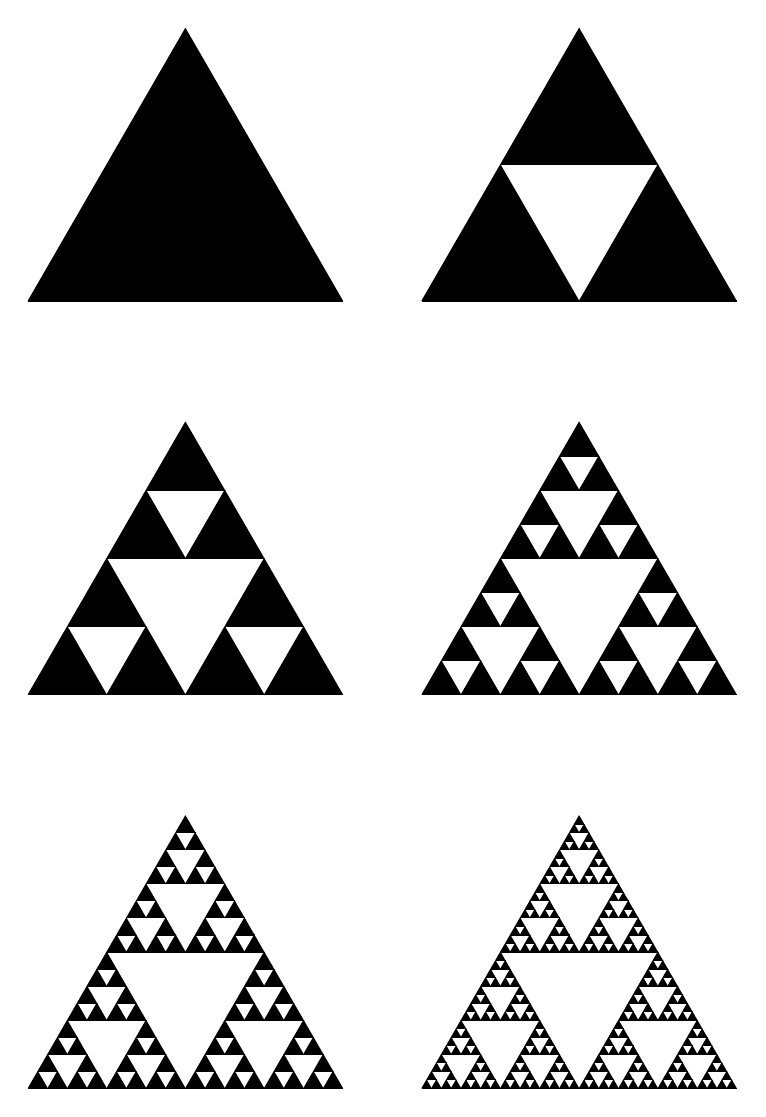
\begin{tikzpicture}
\tikzmath{
% Define the recursive function sierpinski
function sierpinski(\x, \y, \s, \d) {
if (\d == 0) then {
% Draw a triangle lower left corner at (\x, \y), length \s
{ \Triangle{(\x,\y)}{\s}; };
} else {
% Rescale the length of the sides and choose correct coords
% for the next triangles
\u1 = 0.25*\s;
\u2 = \u1*sqrt(3);
\u3 = 0.5*\s;
sierpinski(\x,\y,\u3,\d-1);
sierpinski(\x+\u3,\y,\u3,\d-1);
sierpinski(\x+\u1,\y+\u2,\u3,\d-1);
};
};
% Let the length of the sides of the base triangle be 4, and generate 6 figures
\S = 4;
for \d in {0,...,5}{
% To situate all plots nicely under and next to each other, define the coords
% of the lower left corners preemptively
\x = (\S+1)*mod(\d,2);
\y = int(\d/2) * (\S+1);
sierpinski(\x,-\y,\S,\d);
};
}
\end{tikzpicture}
\end{document}
